\documentclass{beamer}
\mode<presentation>
\usepackage{amsmath}
\usepackage{amssymb}
%\usepackage{advdate}
\usepackage{graphicx}
\graphicspath{{../Figs/}}
\usepackage{adjustbox}
\usepackage{subcaption}
\usepackage{enumitem}
\usepackage{multicol}
\usepackage{mathtools}
\usepackage{listings}
\usepackage{url}
\def\UrlBreaks{\do\/\do-}
\usetheme{Boadilla}
\usecolortheme{lily}
\setbeamertemplate{footline}
{
  \leavevmode%
  \hbox{%
  \begin{beamercolorbox}[wd=\paperwidth,ht=2.25ex,dp=1ex,right]{author in head/foot}%
    \insertframenumber{} / \inserttotalframenumber\hspace*{2ex} 
  \end{beamercolorbox}}%
  \vskip0pt%
}
\setbeamertemplate{navigation symbols}{}
\let\solution\relax
\usepackage{gvv}
\lstset{
%language=C,
frame=single, 
breaklines=true,
columns=fullflexible
}

\numberwithin{equation}{section}
\begin{document}


\title{4.7.63}
\author{AI25BTECH11002 - Ayush Sunil Labhade}
{\let\newpage\relax\maketitle}

\textbf{Question}:
Find the equation of plane that contains the point $\brak{1,-1,2}$ and is perpendicular to each of the planes 2x+3y-2z=5 and x+2y-3z=8. 	


\textbf{Solution:}

Let the equation of plane be:
\begin{align}
	\vec{n}^T\vec{x} = 1
\end{align}
Since the plane contains the point  $\vec{A} = \myvec{1\\-1\\2}$, 
\begin{align}
	\vec{n}^T\vec{A} = 1
\end{align}
Also since the plane is perpendicular to the planes 2x+3y-2z=5 and x+2y-3z=8
\begin{align}
	\vec{n}^T\vec{B} = 0 \newline \quad
\vec{B} = \myvec{2 \\ 3 \\ -2} \quad 
\end{align}
\begin{align}
	\vec{n}^T\vec{C} = 0 \newline \quad 
\vec{C} = \myvec{1 \\ 2 \\ -3}
\end{align}
We can rewrite it as
\begin{align}
	\brak{\vec{A} \vec{B} \vec{C}}^T\vec{n}=\myvec{1 \\ 0 \\0}
\end{align}
Forming the augmented matrix:
\begin{align}
	\augvec{3}{1}{1 & -1 & 2 & 1 \\ 2 & 3 & -2 & 0\\1 & 2 & -3& 0}
\end{align}
On row reducing we get,
\begin{align}
	\augvec{3}{1}{1 & 0 & 0 & -\tfrac{5}{7}\\
0 & 1 & 0 & \tfrac{4}{7}\\
0 & 0 & 1 & \tfrac{1}{7}}
\end{align}
	
\begin{align}
	\vec{n} = \myvec{-5 \\ 4 \\ 1}
\end{align}

$\therefore$ the required equation is
\begin{align}
		\myvec{-5&4&1}\vec{x} = 7
\end{align}
		

Graph:
\begin{figure}[H]
    \centering
    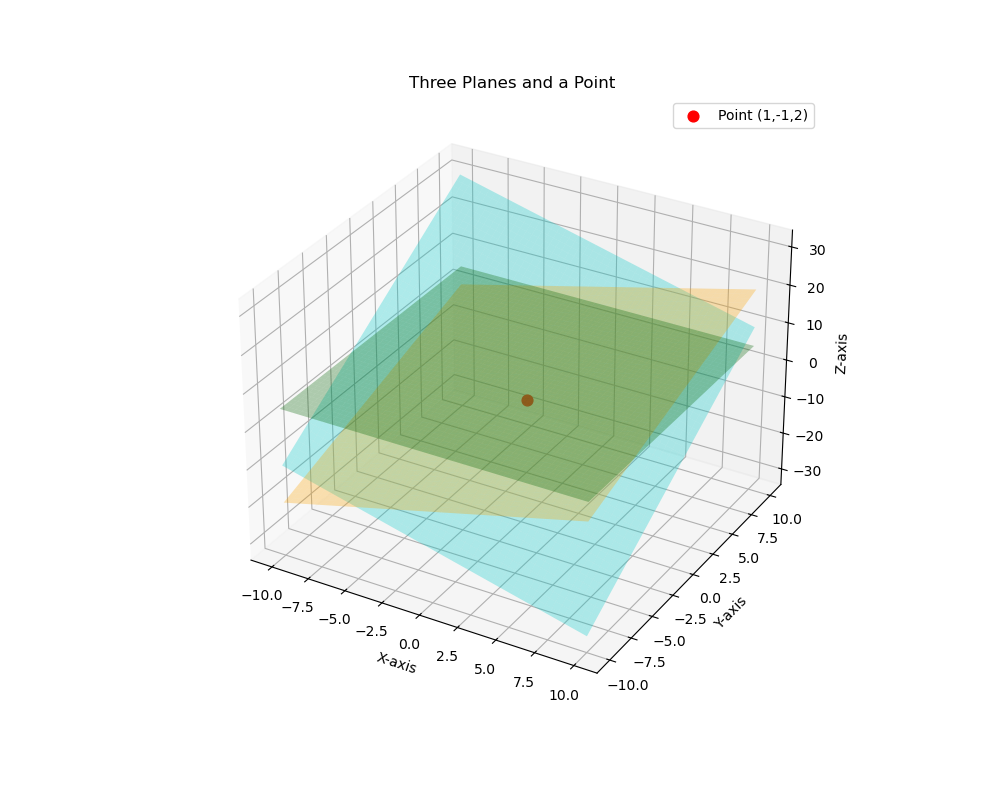
\includegraphics[scale=0.5]{plot}
    \caption{}
    \label{fig:plot}
\end{figure}
\end{document}
